\documentclass[tikz,border=5pt]{standalone}
\usepackage{amsmath}
\usetikzlibrary{arrows.meta,calc,positioning}

\definecolor{obsfill}{HTML}{DDEBF7}
\definecolor{obsline}{HTML}{2F5597}
\definecolor{basefill}{HTML}{EFEFEF}
\definecolor{baseline}{HTML}{595959}
\definecolor{resfill}{HTML}{FBE5D6}
\definecolor{resline}{HTML}{C55A11}
\definecolor{corrfill}{HTML}{E2F0D9}
\definecolor{corrline}{HTML}{548235}
\definecolor{evalline}{HTML}{404040}
\definecolor{flowline}{HTML}{333333}

\begin{document}
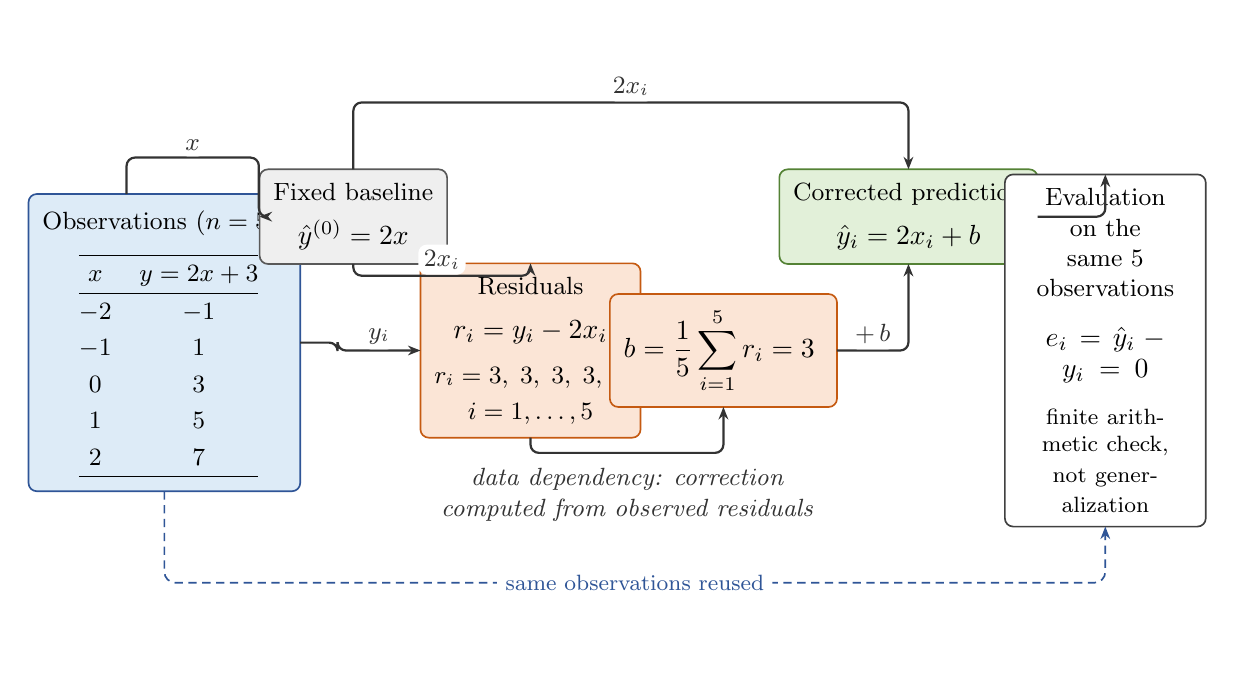
\begin{tikzpicture}[
    font=\fontsize{9}{11}\selectfont,
    box/.style={
        rectangle,
        rounded corners=3pt,
        line width=0.6pt,
        align=center,
        inner sep=5pt,
        outer sep=0pt
    },
    observed/.style={box,fill=obsfill,draw=obsline},
    baselinebox/.style={box,fill=basefill,draw=baseline},
    residualbox/.style={box,fill=resfill,draw=resline},
    correctedbox/.style={box,fill=corrfill,draw=corrline},
    evaluationbox/.style={box,fill=white,draw=evalline},
    flow/.style={
        draw=flowline,
        line width=0.8pt,
        -{Stealth[length=4.5pt,width=3.5pt]},
        rounded corners=3pt
    },
    reuse/.style={
        draw=obsline,
        line width=0.6pt,
        dash pattern=on 3pt off 2pt,
        -{Stealth[length=4.5pt,width=3.5pt]},
        rounded corners=4pt
    },
    arrowlabel/.style={
        font=\fontsize{9}{11}\selectfont,
        fill=white,
        inner sep=2pt,
        text=flowline
    }
]

% White landscape canvas with a 16:9 drawing area.
\path[fill=white] (0,0) rectangle (14.4,8.1);

% Observation table: column centers also define the outgoing data ports.
\node[observed,minimum width=2.15cm,minimum height=3.25cm]
    (obs) at (1.10,4.10) {%
    \begin{tabular}{@{}c@{}}
        Observations ($n=5$)\\[6pt]
        \begingroup
        \renewcommand{\arraystretch}{1.2}
        \setlength{\tabcolsep}{5pt}
        \begin{tabular}{@{}cc@{}}
            \hline
            $x$ & $y=2x+3$\\
            \hline
            $-2$ & $-1$\\
            $-1$ & $1$\\
            $0$  & $3$\\
            $1$  & $5$\\
            $2$  & $7$\\
            \hline
        \end{tabular}
        \endgroup
    \end{tabular}
};

\node[baselinebox,minimum width=1.90cm,minimum height=1.10cm]
    (base) at (3.50,5.70) {%
    Fixed baseline\\[5pt]
    {\fontsize{10}{12}\selectfont $\hat{y}^{(0)}=2x$}
};

\node[residualbox,minimum width=2.30cm,minimum height=1.45cm]
    (resid) at (5.75,4.00) {%
    Residuals\\[5pt]
    {\fontsize{10}{12}\selectfont $r_i=y_i-2x_i$}\\[5pt]
    $r_i=3,\;3,\;3,\;3,\;3$\\[2pt]
    $i=1,\dots,5$
};

\node[residualbox,minimum width=2.05cm,minimum height=1.10cm]
    (bval) at (8.20,4.00) {%
    {\fontsize{10}{12}\selectfont
        $\displaystyle b=\frac{1}{5}\sum_{i=1}^{5}r_i=3$}
};

\node[correctedbox,minimum width=2.25cm,minimum height=1.15cm]
    (corr) at (10.55,5.70) {%
    Corrected prediction\\[5pt]
    {\fontsize{10}{12}\selectfont $\hat{y}_i=2x_i+b$}
};

\node[evaluationbox,text width=2.20cm,minimum height=2.05cm]
    (eval) at (13.05,4.00) {%
    Evaluation on the\\
    same 5 observations\\[7pt]
    {\fontsize{10}{12}\selectfont $e_i=\hat{y}_i-y_i=0$}\\[7pt]
    {\fontsize{8}{10}\selectfont
        finite arithmetic check,\\
        not generalization}
};

% x exits above its observation-table column.
\coordinate (obsx) at ($(obs.north)+(-0.48,0)$);
\draw[flow]
    (obsx) -- (0.62,6.45)
    -- node[arrowlabel,above] {$x$} (2.30,6.45)
    -- (2.30,5.70) -- (base.west);

% Observed y values feed residual computation.
\draw[flow]
    (obs.east) -- (3.30,4.10)
    -- (3.30,4.00)
    -- node[arrowlabel,above] {$y_i$} (resid.west);

% Baseline values feed residual computation.
\draw[flow]
    (base.south) -- (3.50,4.95)
    -- node[arrowlabel,above] {$2x_i$} (5.75,4.95)
    -- (resid.north);

% The baseline also feeds the corrected prediction along the upper route.
\draw[flow]
    (base.north) -- (3.50,7.15)
    -- node[arrowlabel,above] {$2x_i$} (10.55,7.15)
    -- (corr.north);

% The annotated dependency is given its own spacious lower route.
\draw[flow]
    (resid.south) -- (5.75,2.70)
    -- (8.20,2.70) -- (bval.south);

\node[
    align=center,
    text=flowline,
    font=\fontsize{9}{11}\selectfont\itshape,
    anchor=north,
    inner sep=2pt
] at (6.975,2.58) {%
    data dependency: correction\\
    computed from observed residuals
};

% Add the fitted scalar correction.
\draw[flow]
    (bval.east)
    -- node[arrowlabel,above] {$+\,b$} (10.55,4.00)
    -- (corr.south);

% Corrected values enter the arithmetic evaluation.
\draw[flow]
    (corr.east) -- (13.05,5.70) -- (eval.north);

% Reuse of the same observations is visually distinct from computation.
\draw[reuse]
    (obs.south) -- (1.10,1.05)
    -- node[
        midway,
        fill=white,
        inner sep=3pt,
        text=obsline,
        font=\fontsize{8.5}{10}\selectfont
    ] {same observations reused}
    (13.05,1.05) -- (eval.south);

\end{tikzpicture}
\end{document}